\section{Introduction}
\label{sec:introduction}
The proliferation of remote sensing equipment (such as radars and satellites); networked sensors and monitoring equipment; and commercial applications such as mapping services, location-based recommendation services and sales tracking have resulted in the exponential growth of spatiotemporal data. Spatiotemporal data comprise observations where in addition to the features of interest (such as humidity, air quality, disease prevalence, sales, etc) both the spatial and chronological components representing the time and location where measurements were made are available. 

Spatiotemporal data includes a wealth of information that can be used to inform: decision making, scientific modeling and simulations, and resource allocations in several domains.  These domains include atmospheric science, epidemiology, environmental science, geosciences, smart-city settings, and commercial applications.  Querying these voluminous datasets and the expressiveness of these queries underpin efficiency in these settings. To be effective, regardless of the data volumes, the query evaluations must be in real-time and at high-throughput meaning a large number of queries must be evaluated per second. 

Spatiotemporal datasets are naturally multidimensional with multiple features of interest being reported/recorded continually for a particular timestamp and geolocation. The values associated with these features are continually changing --- in other words, the feature space represented by these datasets are continually evolving. 

Queries specified over these datasets may have wide range of characteristics encompassing the frequency at which they are evaluated, and the spatiotemporal scope associated with these queries. The crux of this paper is to support query evaluations over continually arriving observational data. The queries may be continuous or discrete, involve sliding windows, and varying geospatial scopes.

\subsection{Challenges}
Support for real-time evaluation of queries – discrete and continuous – over a feature space that is continually evolving introduces unique challenges. These include:
\begin{itemize}
\item   Data volumes: It is infeasible to store all the observational data. This is especially true if the arrival rates outpace the rate at which data can be written to disk.
\item   Data arrival rates: The data may arrive continually and at high rates. Furthermore, this rate of arrivals may change over time.
\item   Accuracy: Queries specified by the user — continuous or one-time — must be accurate.
\item   Continuous query evaluations: Users should be able to register query evaluations over the observational space that must be continually evaluated.
\item   Spatiotemporal data characteristics: Queries that are issued by a user may target spatiotemporal properties associated with these observations. For e.g., a user may be interested in feature characteristics for a geospatial location at a particular daily interval (say 2:00-4:00 pm) over a particular chronological range (say, 2-3 months)
\end{itemize}

\subsection{Research Questions}
\begin{enumerate}
\item   How can we generate compact, memory-resident (i.e. the sketch) representations of the observational space? The sketch must be amenable to fast, continuous updates to ensure that the sketch is representative of the observational space.
\item   How can we scale effectively in situations where the observations arrive at a rate faster than the rate at which the sketch can be updated? The density and arrival rates for observations vary based on the geospatial characteristics of the data. For example, in a smart-city setting NYC would like have a far higher rate of observations than a mid-sized city like Denver, which in turn would have a far higher rate of observations than a small city such as Fort Collins.
\item   How can we effectively account for the spatiotemporal attributes associated with both the observations and the queries specified by the users? This spans the generation and updates of the sketch, scaling in response to high data arrival rates, and the evaluation of the queries.
\item   How can we ensure high-throughputs in the assimilation of observations, updates to the sketch, and query evaluations? A particular challenge is preservation of accuracy in query evaluations despite high data arrivals, scaling in response to changes in system load, and concurrent query evaluations.  This encompasses using horizontal scaling to proactively alleviate hotspots, maintaining a distributed representation of the sketch, and effective distribution, targeting, and combining of query evaluations.
\end{enumerate}

\subsection{Methodology}
Our methodology targets: (1) creation of the sketch, (2) updating the sketch in response to data arrivals, (3) identifying performance hotspots via targeted alleviation of performance hotspots, (4) support for splitting and fusing a sketch, and (5) dynamic creation of distributed sketch. (6) using the distributed sketch to perform query evaluations, and (7) achieve high-throughput by minimizing synchronization between different portions of the distributed sketch. 

Extract metadata from observations
Organize this metadata in an in-memory sketch.

Our sketch supports 3 key features. Specifically, the sketch (1) maintains a compact representation of the observations seen so far, (2) is amenable to splitting and fusing, and (3) supports query evaluations  including specification of sliding window sizes and geospatial scopes to support exploring properties of the observational space.  The sketch is naturally amenable to support distributed representations; with each node within the cluster holding information about the observational space. The distributed representation of the sketch is that of a dynamic, continually-updated in-memory store.

There are several advantages to a distributed representation of the sketch. (1) It allows us to maintain a richer (finer-grained) representation  of the feature space. (2) it improves accuracy during query evaluations, (3) supports multiple, concurrent query evaluations with each node evaluating queries independently.

Furthermore, at each node we dynamically adjust the representativeness of the sketch. There are two options here: bias towards the recent past or equal representations. In the former approach, the sketch targets finer-grained representations of observations in the recent past, and progressively coarser grained representations for the farther past. This scheme ensures that the apportioning of the available memory for the sketch is proportional to the time-intervals under consideration. For example, last 3 minutes, last 3 hours, last 3 days, last 3 months, last 3 years, and last 3 decades would have equal memory footprints.  In the latter approach, the sketch maintains a coarser-grained representations at each node.

The sketch scales (up or down) dynamically to cope with data arrival rates. At each node, the expressiveness of the sketch can be tuned dynamically based on the available memory. At each node, the sketch continually updates the expressiveness of the portions of the feature space, dynamically reorients the graph-based structure, and minimizes traversals (using Bloom Filters) to support faster evaluations and preserve high-throughput. 

\subsection{Paper Contributions}
In this paper we presented a framework for supporting real-time query evaluations over voluminous, time-series data streams. Our specific contributions include:
\begin{itemize}
\item   Design of the Trident sketch that maintains compact, distributed representations of the observational space. At each node, the sketch supports dynamic reorientations to conserve memory and support faster query evaluations.
\item   Support for dynamic scaling of the sketch in response to the data arrival rates. Upscaling operations support targeted alleviation of hotspots. Only geographic locations that are observing high data arrival rates are scale. The framework manages the complexity of identifying these hotspots, splitting the particular portion of the sketch, and migrating relevant portions of the sketch. Most importantly, the framework achieves this while maintaining acceptable levels of accuracy in query evaluations.
\item   Support for one-time and continuous evaluations of the observational space. We incorporate support for CQL queries. Query evaluations can target arbitrarily sized (chronological) window sizes and geospatial scopes.
\item   Support for high-throughput, distributed evaluation of queries.
To our knowledge, Trident is the first sketch designed specifically for geospatial observational data. We have validated the suitability of our approach through a comprehensive set of benchmarks with real observational data. 
\end{itemize}

\cite{buddhika2016neptune}

\subsection{Paper Organization}
The remainder of this paper is organized as follows...

\subsection{Stream Partitioning}
We use the Geohash~algorithm~\cite{geohash} to balance load and partition incoming data streams across processing resources. Geohash divides the earth into a hierarchy of bounding boxes identified by Base 32 strings; the longer the Geohash string, the more precise the bounding box. Figure~\ref{fig:geohash} illustrates this hierarchy; most of the western United States and Mexico are contained within the bounding box described by Geohash string \emph{9}, while \emph{9Q} encompasses parts of California, Nevada, Arizona, and Utah. The bounding box \emph{9Q9K} (highlighted in red) contains San Jose, California. This hierarchical representation enables \textsc{Rivulet} to cope with both low- and high-density regions. For instance, several resources may be tasked with managing streams originating in and around the San Francisco region, while the entirety of Yosemite National Park could fall under the purview of a single node.

\begin{figure}
    \centerline{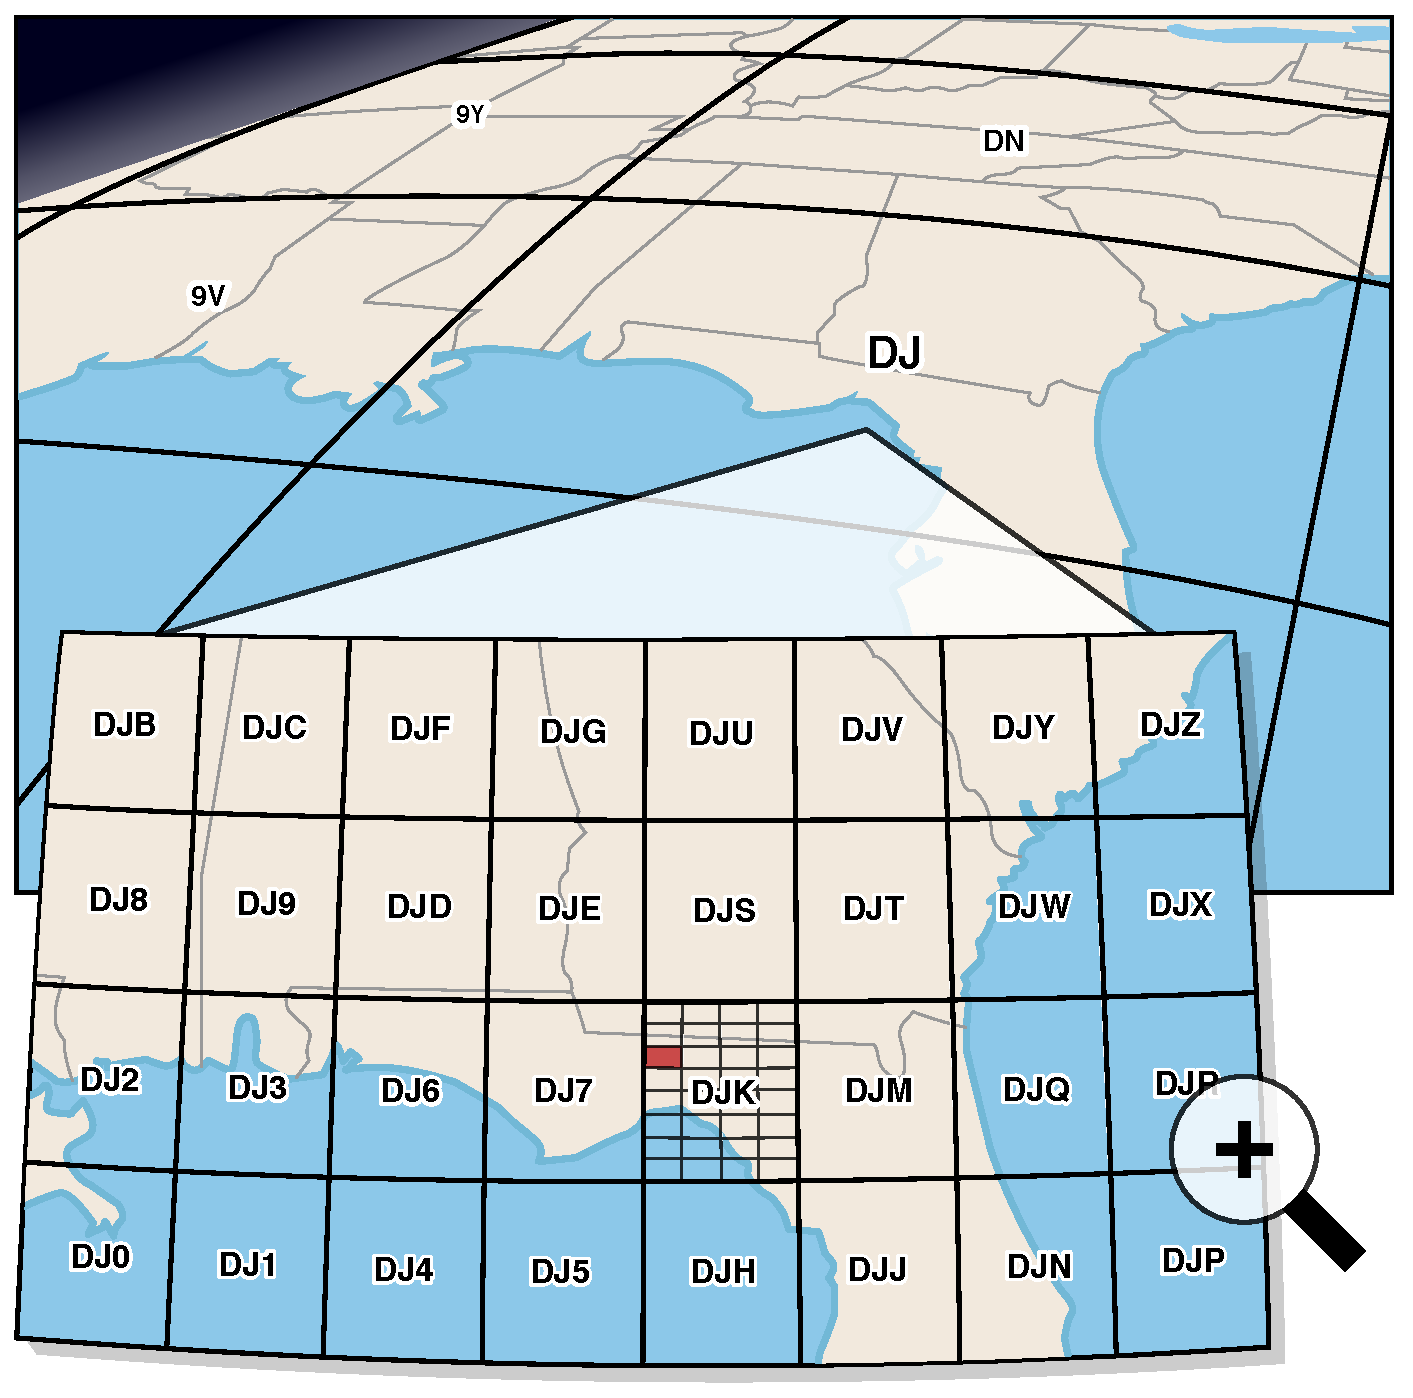
\includegraphics[width=3.5in]{figures/geohash.pdf}}
    \caption{A demonstration of the Geohash algorithm. Each additional character in a Geohash string describes a finer-grained region; Geohash \emph{9Q} contains a substantial portion of California, USA, while \emph{9Q9K} (highlighted in red) represents a smaller region containing San Jose, California.}
    \label{fig:geohash}
\end{figure}

To achieve fine-grained control over our Geohash partitions, we operate at the bit level rather than Base 32 character level when routing streams. Each bit added to a Geohash string reduces its scope by half, with each character represented by five bits ($2^5 = 32$). In other words, a four-character Geohash string represents 20 spatial subdivisions. This property allows us to manage and allocate resources across a wide variety of observational densities.

 % This needs to be moved as we get the paper structure finalized

